\documentclass{standalone}
\usepackage{ tikz }
\usepackage{ xparse }
\usepackage{../../../macros}

\begin{document}
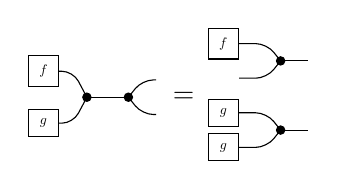
\begin{tikzpicture}[yscale=-1,x=1em,y=1.25em]
        
    \node [draw, anchor=east, minimum width=1.1em] at (6,0.25) {\scalebox{0.5}{$f$}};
    \node [draw, anchor=east, minimum width=1.1em] at (6,1.75) {\scalebox{0.5}{$g$}};
    \draw [rounded corners] (6,0.25) -- (6.5,0.25) -- (7,1);
    \draw [rounded corners] (6,1.75) -- (6.5,1.75) -- (7,1);
    \filldraw (7,1) circle (1.5pt);
    \draw (7,1) -- (8.5,1);
    \filldraw (8.5,1) circle (1.5pt);
    \draw [rounded corners] (8.5,1) -- (9,0.5) -- (9.5,0.5);
    \draw [rounded corners] (8.5,1) -- (9,1.5) -- (9.5,1.5);

    \node at (10.5,1) {$=$};

    \node [draw, anchor=east, minimum width=1.1em] at (12.5,-0.55) {\scalebox{0.5}{$f$}};
    \node [draw, anchor=east, minimum width=1.1em] at (12.5,1.45) {\scalebox{0.5}{$g$}};
    \node [draw, anchor=east, minimum width=1.1em] at (12.5,2.45) {\scalebox{0.5}{$g$}};    

    \draw [rounded corners] (12.5, -0.55) -- (13.5, -0.55) -- (14,-0.05);
    \draw [rounded corners] (12.5, 0.45) -- (13.5, 0.45) -- (14,-0.05);
    \filldraw (14,-0.05) circle (1.5pt);
    \draw (14,-0.05) -- (15, -0.05);

    \draw [rounded corners] (12.5, 1.45) -- (13.5, 1.45) -- (14, 1.95);
    \draw [rounded corners] (12.5, 2.45) -- (13.5, 2.45) -- (14, 1.95);
    \filldraw (14,1.95) circle (1.5pt);
    \draw (14,1.95) -- (15, 1.95);

\end{tikzpicture}
\end{document}